\chapter{Game Description}

In this strategic puzzle game, players compete to create stunning stained glass windows using colorful 
dice and complete different patterns. Each player is tasked with carefully selecting and placing dice to fulfill 
specific pattern requirements while navigating constraints and maximizing their score.

For a comprehensive understanding of the game rules and mechanics, the reader should refer to 
the official rule book provided by the publisher. The rule book  \textcite{Sagradarulesbook} serves as the 
authoritative source for setup instructions, gameplay rules and scoring criteria.

While the official rule book offers a comprehensive overview of Sagrada's gameplay mechanics, it does not 
delve into detailed descriptions of specific components or strategies. In the following sections, I aim 
to fill in the gaps left by the rule book, offering detailed descriptions and strategic insights into 
various aspects of Sagrada's gameplay.



\newcommand{\cmark}{\ding{51}}%
\newcommand{\xmark}{\ding{55}}%

\section{Tool Cards (TC)}
Tool Cards provide unique actions that players can take throughout the game to manipulate dice placements, 
modify their boards, or gain additional benefits. One important attribute of a Tool Card is whether it shifts turns or not.
The ones that don't shift the turn allow the players to make either a passing move or a die-placing move after using the Tool Card.
The following table illustrates the 12 different Tool Cards present in the game marking the ones that shift turns with a \cmark and
the ones that do not shift turns with a \xmark :


\newcolumntype{Y}{>{\hsize=0.6\hsize}X}
\setlength{\extrarowheight}{13pt}

\begin{tabularx}{\textwidth}{>{\bfseries}Y|X}
  Name (Shifts turns) & \textbf{Description} \\ 
  \hline
  1. Copper Foil Furnisher(\xmark) & Allows a player to move a die that is already placed on the board to another position ignoring the shade restriction of the destination space. The player must obey all other placement restrictions. \\  
  2. Eglomise Brush(\xmark) & Allows a player to move a die that is already placed on the board to another position ignoring the color restriction of the destination space. The player must obey all other placement restrictions. \\  
  3. Cork-backed Straightedge(\cmark) & Allows a player to place a die on the board to a space that is not adjacent to any other dice. \\  
  4. Flux Brush(\cmark) & Allows a player to re-roll a die from the Draft Pool. The die must be placed on the board if there is any space where the die could be placed with the re-rolled value. Otherwise, the die is returned to the Draft Pool. \\ 
  5. Flux Remover(\cmark) & Allows a player to choose a die from the Draft Pool, swap it with a random die from the Dice Bag and choose the new die's value. The die must be placed on the board if there is any space where the die could be placed with the re-rolled value. Otherwise, the die is returned to the Draft Pool. \\ 
  6. Glazing Hammer(\xmark) & Allows a player to re-roll all dice in the Draft Pool. This Tool Card may only be used on the second turn of a player before drafting.\\  
  7. Grinding Stone(\cmark) & Allows a player to flip a die from the Draft Pool to its opposite side (6 flips to 1, 5 flips to 2, 4 flips to 3). The player must place the flipped die on the board. The die can be flipped only if it is placeable on the board after the flipping. \\
  8. Grozing Pliers(\cmark) & Allows a player to increase or decrease the value of a die from the Draft Pool by 1. 1 cannot be decreased to 6 and 6 cannot be increased to 1. The player must place the flipped die on the board. The die can be flipped only if it is placeable on the board after the flipping.\\
  9. Lathekin(\xmark) & Allows the player to move exactly two dice that are already placed on the board to other positions obeying all placement restrictions. \\ 
  10. Lens Cutter(\cmark) & Allows a player to swap a die from the Draft Pool with one from the Round Track. After swapping the dice, the new die has to be placed on the board. \\
  11. Running Pliers(\xmark) & Allows a player to immediately draft a die after their first turn. This means that using this Tool Card allows the player to move twice in a row. \\ 
  12. Tap Wheel(\xmark) & Allows a player to move one or two dice of the same color that are already placed on the board to a new position. The color of the dice must match the color of a die on the Round Track. The player must obey all the placement restrictions.
\end{tabularx}

I am using the appellation ``relocating tool cards'' multiple times in the text referring to Tool Cards that allow a player to move one or more dice that are already placed 
on the board to a new position. Namely, these are  \textbf{the Copper Foil Furnisher}, \textbf{the Eglomise Brush}, \textbf{the Tap Wheel} and \textbf{the Lathekin} Tool Cards.


\section{Public Objective Cards (PuOC)}
Public Objective Cards represent shared goals that all players strive to achieve throughout the game. These cards provide additional 
challenges and opportunities for players to earn points based on completing specific patterns. For each completed pattern, the player
receives the satisfaction value that belongs to the Public Objective Card. There are 10 different Public Objective Cards:

\begin{tabularx}{\textwidth}{>{\bfseries}l|X}
  Name & \textbf{Description} \\ 
  \hline
  1. Color Diagonal & Awards one point for each die that has a diagonal neighbor of the same color, regardless of the specific colors involved. \\  
  2. Column Color Variety &  The pattern is fulfilled when a given column contains dice whose colors are all different, ensuring that all spaces within the column are occupied by a die. Completing a pattern is worth 5 points.\\
  3. Column Shade Variety & The pattern is fulfilled when a given column contains dice whose shades are all different, ensuring that all spaces within the column are occupied by a die. Completing a pattern is worth 4 points.\\  
  4. Ligh Shades & Awards two points for every pair of dice with a value of 1 and a value of 2. The position of the dice does not matter.\\ 
  5. Medium Shades & Awards two points for every pair of dice with a value of 3 and a value of 4. The position of the dice does not matter.\\ 
  6. Deep Shades & Awards two points for every pair of dice with a value of 5 and a value of 6. The position of the dice does not matter.\\  
  7. Row Color Variety & The pattern is fulfilled when a given row contains dice of different colors, ensuring that all spaces within the row are occupied by a die. Completing a pattern is worth 6 points.\\
  8. Row Shade Variety & The pattern is fulfilled when a given row contains dice of different shades, ensuring that all spaces within the row are occupied by a die. Completing a pattern is worth 5 points.\\
  9. Color Variety & Awards four points for every set of 1 die of each color. The position of the dice does not matter.\\ 
  10. Shade Variety & Awards four points for every set of 1 die of each shade. The position of the dice does not matter.\\
 \end{tabularx}



\section{Window Pattern Cards (WPC)}

After drafting all the Tool Cards, Public Objective Cards and Private Objective Cards, the game continues with every player choosing a Window
Pattern Card. These cards serve as the basic layout of each player's boards. Every space contains a shade restriction,
a color restriction or no restriction at all. If a space contains a restriction, only dice with matching shades/colors can be placed on it.
To every Window Pattern Card belongs a difficulty number which is given to the player in the form of Favor Tokens. There are the following 
24 Window Pattern Card in the game - the difficulty number is represented by the white circles in the lower right corner of the Window Pattern Cards:

\centerline{\mbox{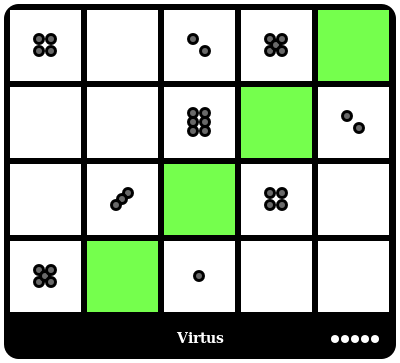
\includegraphics[width=75mm]{img/WPC/Virtus.png}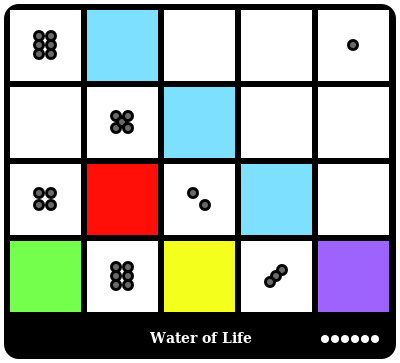
\includegraphics[width=75mm]{img/WPC/WaterofLife.png}}}
\centerline{\mbox{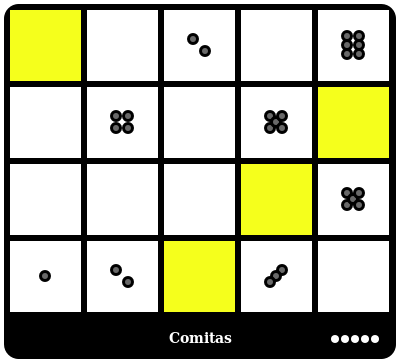
\includegraphics[width=75mm]{img/WPC/Comitas.png}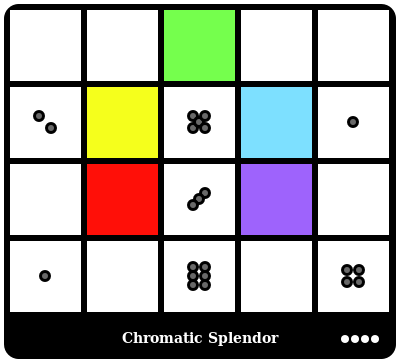
\includegraphics[width=75mm]{img/WPC/ChromaticSplendor.png}}}
\centerline{\mbox{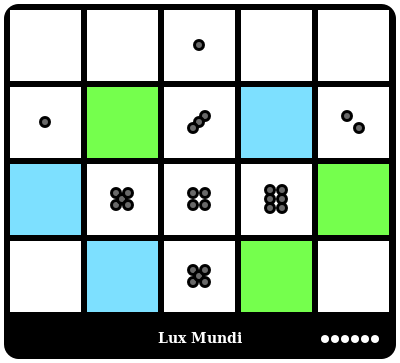
\includegraphics[width=75mm]{img/WPC/LuxMundi.png}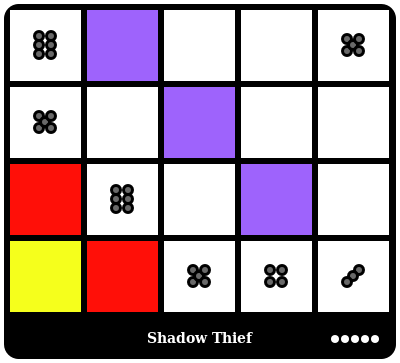
\includegraphics[width=75mm]{img/WPC/ShadowThief.png}}}
\centerline{\mbox{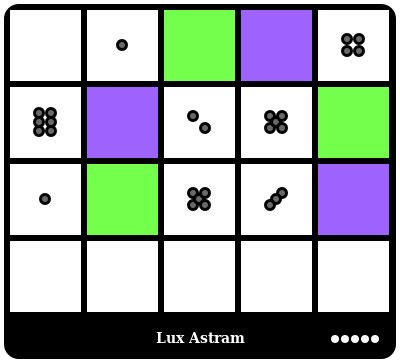
\includegraphics[width=75mm]{img/WPC/LuxAstram.png}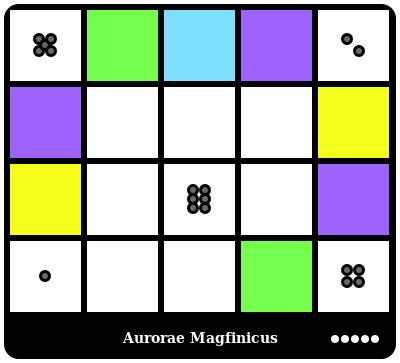
\includegraphics[width=75mm]{img/WPC/AuroraeMagfinicus.png}}}
\centerline{\mbox{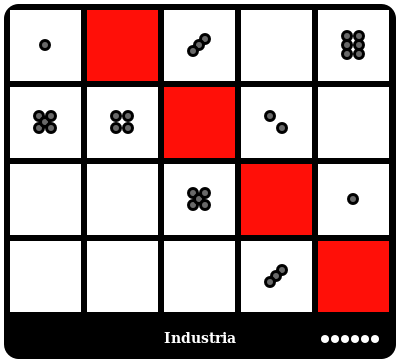
\includegraphics[width=75mm]{img/WPC/Industria.png}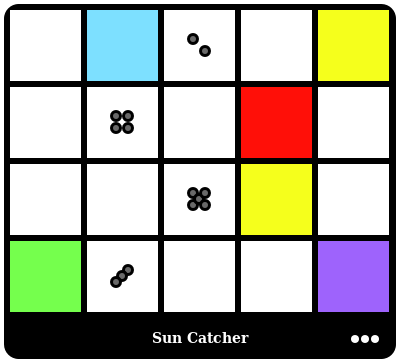
\includegraphics[width=75mm]{img/WPC/SunCatcher.png}}}
\centerline{\mbox{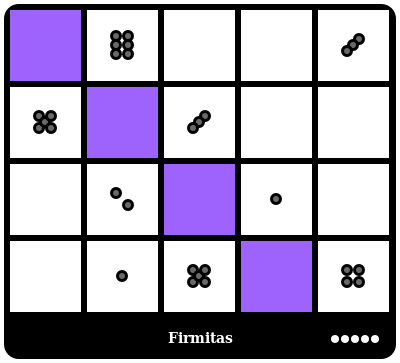
\includegraphics[width=75mm]{img/WPC/Firmitas.png}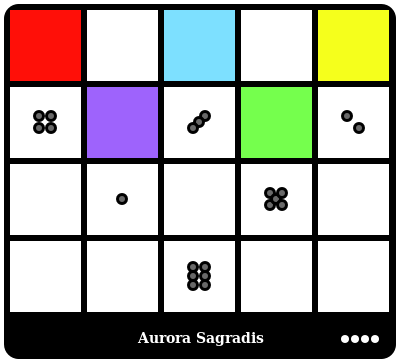
\includegraphics[width=75mm]{img/WPC/AuroraSagradis.png}}}
\centerline{\mbox{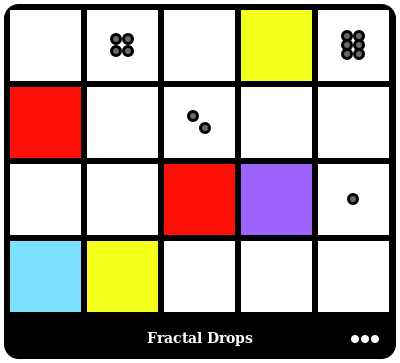
\includegraphics[width=75mm]{img/WPC/FractalDrops.png}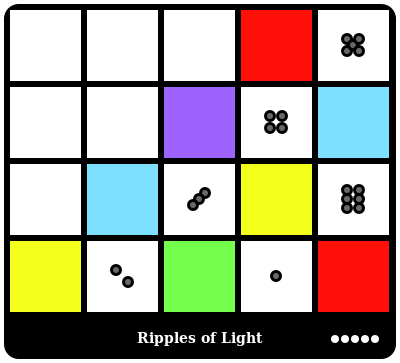
\includegraphics[width=75mm]{img/WPC/RipplesofLight.png}}}
\centerline{\mbox{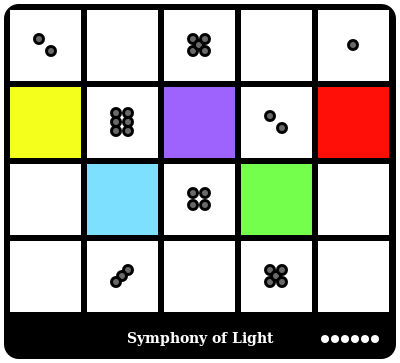
\includegraphics[width=75mm]{img/WPC/SymphonyofLight.png}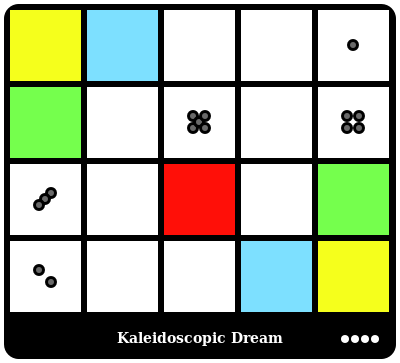
\includegraphics[width=75mm]{img/WPC/KaleidoscopicDream.png}}}
\centerline{\mbox{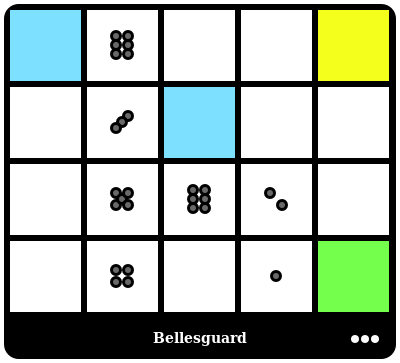
\includegraphics[width=75mm]{img/WPC/Bellesguard.png}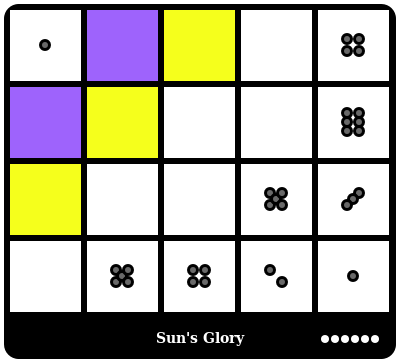
\includegraphics[width=75mm]{img/WPC/Sun'sGlory.png}}}
\centerline{\mbox{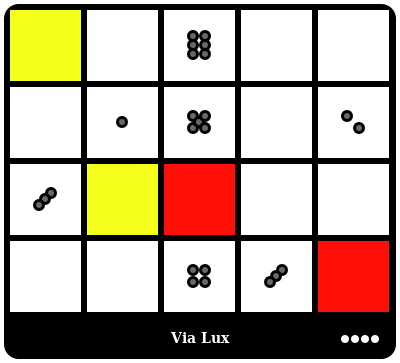
\includegraphics[width=75mm]{img/WPC/ViaLux.png}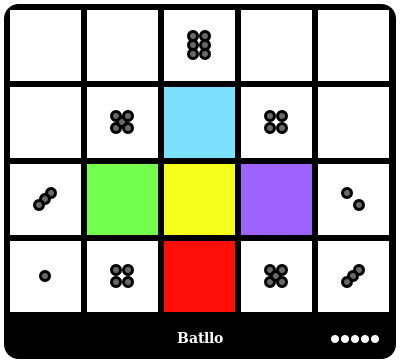
\includegraphics[width=75mm]{img/WPC/Batllo.png}}}
\centerline{\mbox{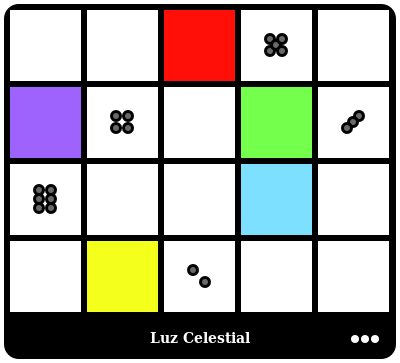
\includegraphics[width=75mm]{img/WPC/LuzCelestial.png}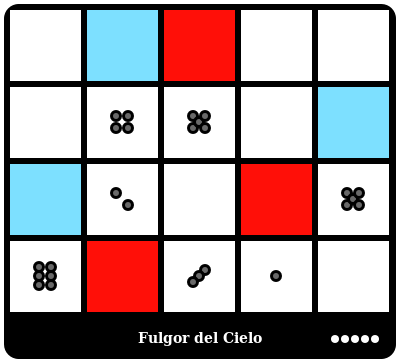
\includegraphics[width=75mm]{img/WPC/FulgordelCielo.png}}}
\centerline{\mbox{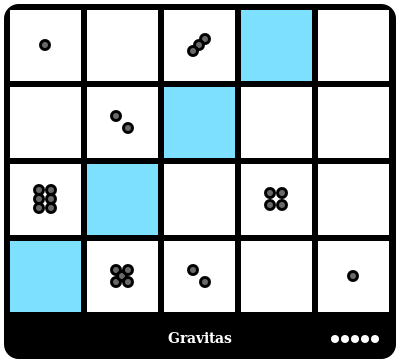
\includegraphics[width=75mm]{img/WPC/Gravitas.png}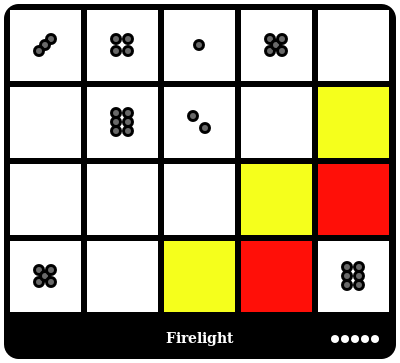
\includegraphics[width=75mm]{img/WPC/Firelight.png}}}
